\documentclass[]{article}
\usepackage{lmodern}
\usepackage{amssymb,amsmath}
\usepackage{ifxetex,ifluatex}
\usepackage{fixltx2e} % provides \textsubscript
\ifnum 0\ifxetex 1\fi\ifluatex 1\fi=0 % if pdftex
  \usepackage[T1]{fontenc}
  \usepackage[utf8]{inputenc}
\else % if luatex or xelatex
  \ifxetex
    \usepackage{mathspec}
    \usepackage{xltxtra,xunicode}
  \else
    \usepackage{fontspec}
  \fi
  \defaultfontfeatures{Mapping=tex-text,Scale=MatchLowercase}
  \newcommand{\euro}{€}
\fi
% use upquote if available, for straight quotes in verbatim environments
\IfFileExists{upquote.sty}{\usepackage{upquote}}{}
% use microtype if available
\IfFileExists{microtype.sty}{\usepackage{microtype}}{}
\usepackage[margin=1in]{geometry}
\usepackage{graphicx}
\makeatletter
\def\maxwidth{\ifdim\Gin@nat@width>\linewidth\linewidth\else\Gin@nat@width\fi}
\def\maxheight{\ifdim\Gin@nat@height>\textheight\textheight\else\Gin@nat@height\fi}
\makeatother
% Scale images if necessary, so that they will not overflow the page
% margins by default, and it is still possible to overwrite the defaults
% using explicit options in \includegraphics[width, height, ...]{}
\setkeys{Gin}{width=\maxwidth,height=\maxheight,keepaspectratio}
\ifxetex
  \usepackage[setpagesize=false, % page size defined by xetex
              unicode=false, % unicode breaks when used with xetex
              xetex]{hyperref}
\else
  \usepackage[unicode=true]{hyperref}
\fi
\hypersetup{breaklinks=true,
            bookmarks=true,
            pdfauthor={Justin Le},
            pdftitle={Tries with Recursion Schemes},
            colorlinks=true,
            citecolor=blue,
            urlcolor=blue,
            linkcolor=magenta,
            pdfborder={0 0 0}}
\urlstyle{same}  % don't use monospace font for urls
% Make links footnotes instead of hotlinks:
\renewcommand{\href}[2]{#2\footnote{\url{#1}}}
\setlength{\parindent}{0pt}
\setlength{\parskip}{6pt plus 2pt minus 1pt}
\setlength{\emergencystretch}{3em}  % prevent overfull lines
\setcounter{secnumdepth}{0}

\title{Tries with Recursion Schemes}
\author{Justin Le}

\begin{document}
\maketitle

\emph{Originally posted on
\textbf{\href{https://blog.jle.im/entry/tries-with-recursion-schemes.html}{in
Code}}.}

Not too long ago, I was browsing the
\href{https://www.reddit.com/r/PrequelMemes}{prequel memes subreddit} --- a
community built around creative ways of remixing and re-contextualizing quotes
from the cinematic corpus of the three Star Wars prequel movies --- when I
noticed that a fad was in progress
\href{https://www.reddit.com/r/PrequelMemes/comments/9w59t4/i_expanded_it/}{constructing
tries based on quotes as keys} indexing stills from the movie corresponding to
those quotes.

This inspired me to try playing around with some tries myself, and it gave me an
excuse to play around with
\emph{\href{https://hackage.haskell.org/package/recursion-schemes}{recursion-schemes}}
(one of my favorite Haskell libraries). If you haven't heard about it yet,
\emph{recursion-schemes} (and the similar library
\emph{\href{https://hackage.haskell.org/package/data-fix}{data-fix}}) abstracts
over common recursive functions written on recursive data types. It exploits the
fact that a lot of recursive functions for different recursive data types all
really follow the same pattern and gives us powerful tools for writing cleaner
and safer code.

Recursion schemes is a perfect example of those amazing accidents that happen
throughout the Haskell ecosystem: an extremely ``theoretically beautiful''
abstraction that also happens to be extremely useful for writing industrially
rigorous code.

Tries are a common intermediate-level recursive data type, and recursion-schemes
is a common intermediate-level library. So, as a fun intermediate-level Haskell
project, let's build a trie data type in Haskell based on recursion-schemes, to
see what it has to offer! The resulting data type will definitely not be a
``toy'' --- it'll be something you can actually use to build meme diagrams of
your own!

\hypertarget{trie}{%
\section{Trie}\label{trie}}

A \href{https://en.wikipedia.org/wiki/Trie}{trie} (prefix tree) is a classic
example of a simple yet powerful data type most people encounter in school (I
remember being introduced to it through a project implementing a boggle solver).

Wikipedia has a nice picture:

\begin{figure}
\centering
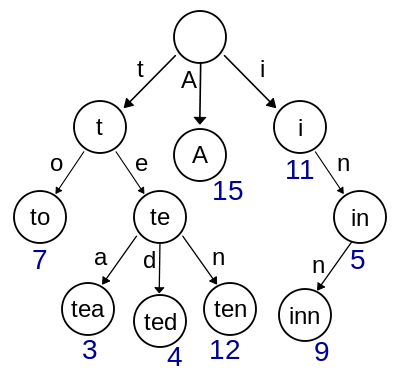
\includegraphics{/img/entries/trie/wiki-trie.png}
\caption{Sample Trie from Wikipedia, indexing lists of Char to Ints}
\end{figure}

\hypertarget{signoff}{%
\section{Signoff}\label{signoff}}

Hi, thanks for reading! You can reach me via email at
\href{mailto:justin@jle.im}{\nolinkurl{justin@jle.im}}, or at twitter at
\href{https://twitter.com/mstk}{@mstk}! This post and all others are published
under the \href{https://creativecommons.org/licenses/by-nc-nd/3.0/}{CC-BY-NC-ND
3.0} license. Corrections and edits via pull request are welcome and encouraged
at \href{https://github.com/mstksg/inCode}{the source repository}.

If you feel inclined, or this post was particularly helpful for you, why not
consider \href{https://www.patreon.com/justinle/overview}{supporting me on
Patreon}, or a \href{bitcoin:3D7rmAYgbDnp4gp4rf22THsGt74fNucPDU}{BTC donation}?
:)

\end{document}
